\subsection{UC3 - Ordinazione collaborativa}\label{usecase:3}

\begin{figure}[H]
    \centering
    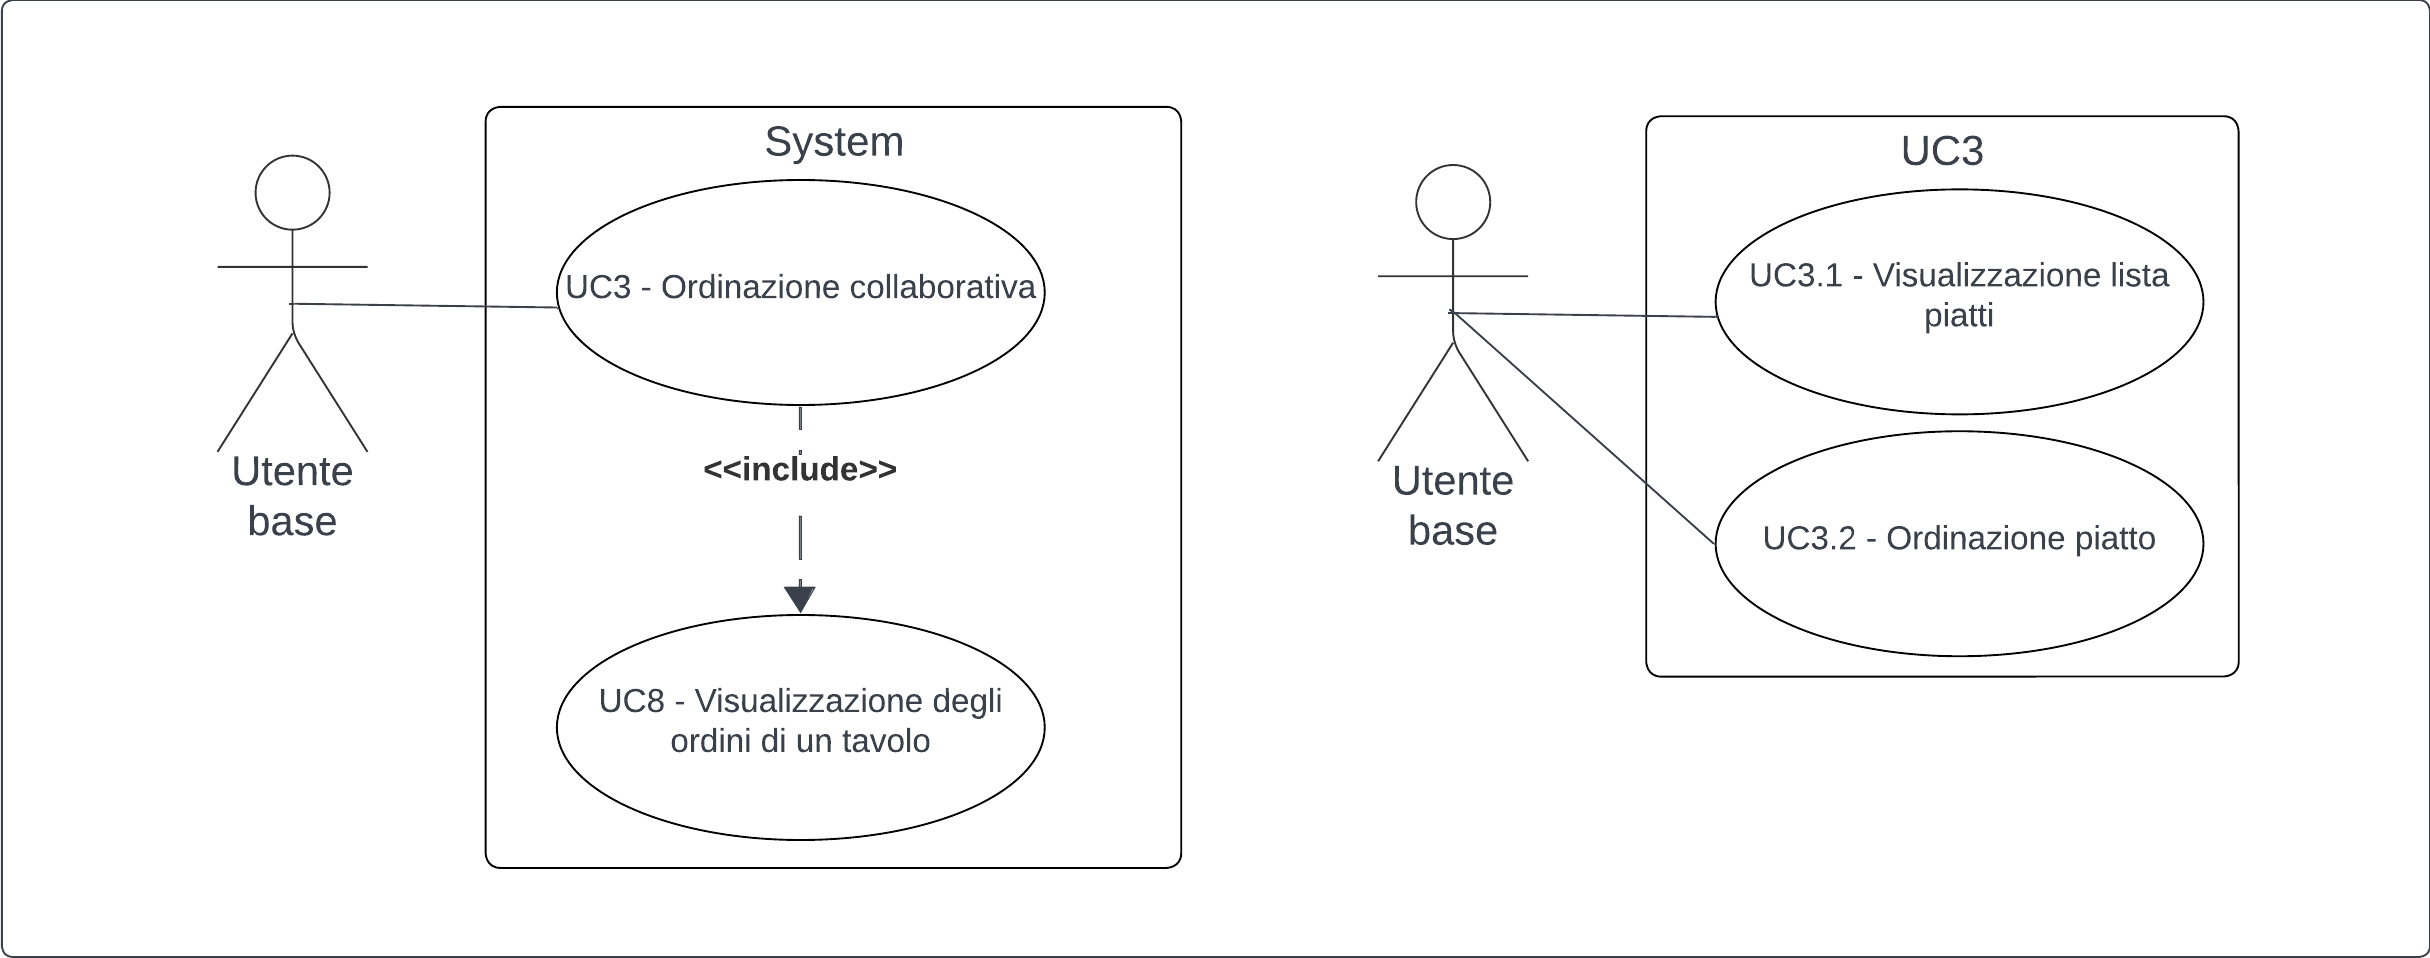
\includegraphics[width=0.9\linewidth]{ucd/UCD3_approfondito.png}
    \caption{Ordinazione collaborativa}
\end{figure}

\textbf{Attori}:
\begin{itemize}
    \item Utente base.
\end{itemize}
\textbf{Precondizioni}:
\begin{itemize}
    \item L'utente è connesso al $\textit{Sistema}_G$; 
    \item L'utente ha prenotato un tavolo (\nameref{usecase:23});
    \item La $\textit{prenotazione}_G$ associata all'$\textit{ordinazione}_G$ è stata accettata dall'utente amministratore del ristorante (\nameref{usecase:19});
    \item Il limite di tempo per l'$\textit{ordinazione}_G$ non è ancora scaduto.
\end{itemize}
\textbf{Postcondizioni}:
\begin{itemize}
    \item L'utente ha confermato $\textit{ordinazione}_G$ delle pietanze associata ad una $\textit{prenotazione}_G$.
\end{itemize}
\textbf{Scenario principale}:
\begin{enumerate}
    \item L'utente crea l'ordine collaborativo:
    \begin{itemize}
    \item L'utente visualizza una lista di piatti da poter ordinare (\nameref{usecase:3_1})
    \item L'utente può scegliere una particolare pietanza e aggiungerla all'ordine (\nameref{usecase:3_2}).
    \end{itemize}
    \item L'utente conferma l'$\textit{ordinazione}_G$;
    \item L'utente può visualizzare il riepilogo del suo ordine e quelli degli altri utenti con cui ha prenotato il tavolo (\nameref{usecase:8});
    \item Il $\textit{sistema}_G$ notifica il ristorante mediante \textit{push-notification}.
\end{enumerate}

\subsubsection{UC3.1 - Visualizzazione lista piatti }\label{usecase:3_1}

\textbf{Attori}:
\begin{itemize}
    \item Utente base.
\end{itemize}
\textbf{Precondizioni}:
\begin{itemize}
    \item L'utente è connesso al $\textit{Sistema}_G$; 
    \item L'utente ha prenotato un tavolo (\nameref{usecase:23});
    \item La $\textit{prenotazione}_G$ associata all'$\textit{ordinazione}_G$ è stata accettata dall'utente amministratore del ristorante (\nameref{usecase:19});
    \item Il limite di tempo per l'$\textit{ordinazione}_G$ non è ancora scaduto.
\end{itemize}
\textbf{Postcondizioni}:
\begin{itemize}
    \item L'utente visualizza una lista di piatti associata al ristorante presso quale è stata fatta la $\textit{prenotazione}_G$.
\end{itemize}
\textbf{Scenario principale}:
\begin{enumerate}
    \item In base al ristorante scelto durante la fase di $\textit{prenotazione}_G$, l'utente visualizza una lista di piatti corrispondenti al menù del ristorante stesso.
\end{enumerate}

\subsubsection{UC3.2 - Ordinazione piatto}\label{usecase:3_2}

\begin{figure}[H]
    \centering
    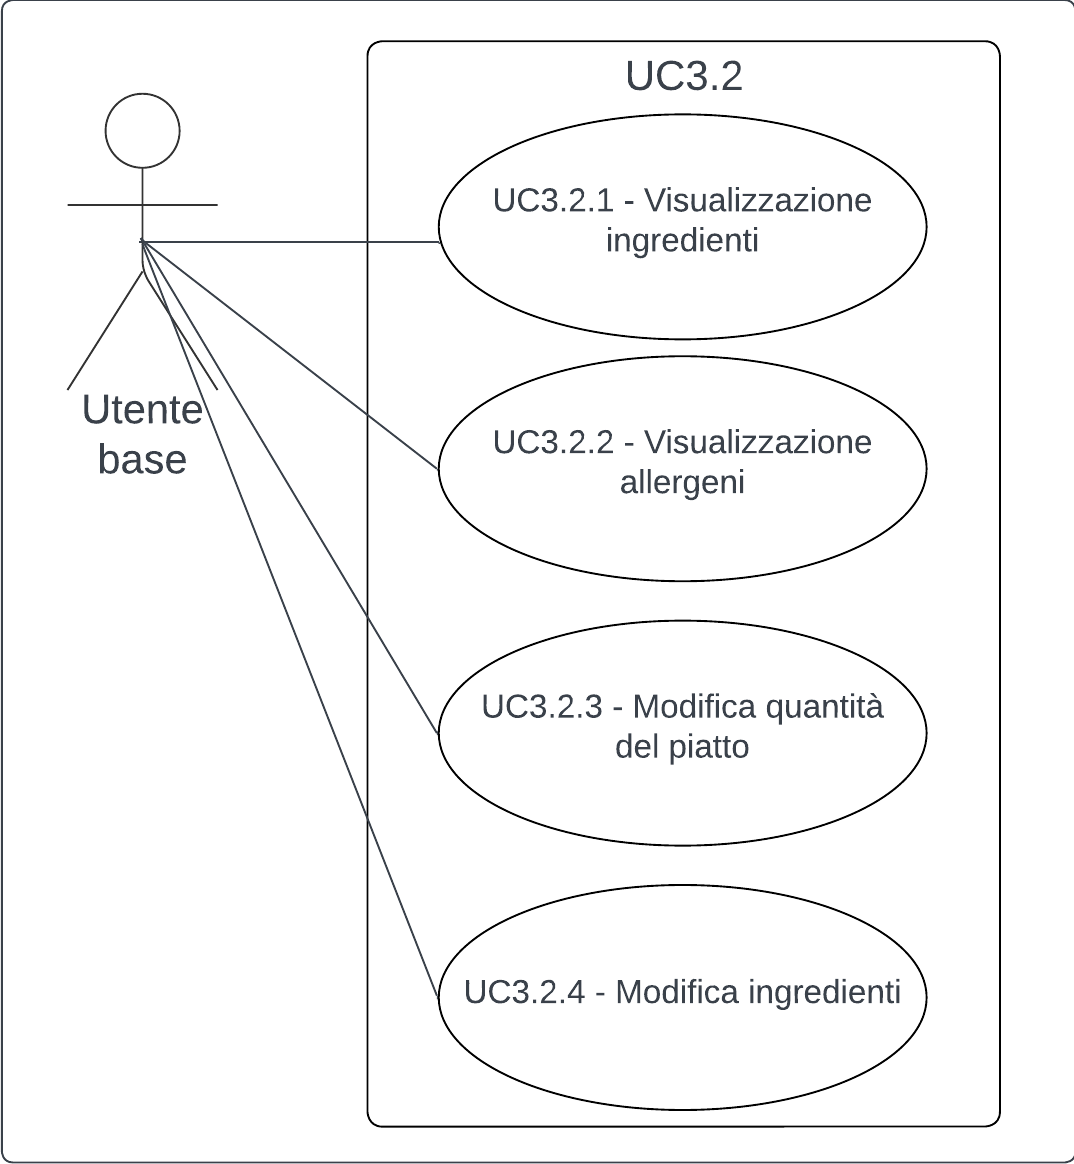
\includegraphics[scale=0.2]{ucd/UCD3.2_finale.png}
    \caption{Ordinazione piatto}
\end{figure}

\textbf{Attori}:
\begin{itemize}
    \item Utente base.
\end{itemize}
\textbf{Precondizioni}:
\begin{itemize}
    \item L'utente è connesso al $\textit{Sistema}_G$; 
    \item L'utente ha prenotato un tavolo (\nameref{usecase:23});
    \item La $\textit{prenotazione}_G$ associata all'$\textit{ordinazione}_G$ è stata accettata dall'utente amministratore del ristorante (\nameref{usecase:19});
    \item Il limite di tempo per l'$\textit{ordinazione}_G$ non è ancora scaduto.
    \item L'utente ha scelto tra la lista delle pietanze una pietanza che vuole aggiungere all'ordine;
\end{itemize}
\textbf{Postcondizioni}:
\begin{itemize}
    \item L'utente ha ordinato il piatto.
\end{itemize}
\textbf{Scenario principale}:
\begin{enumerate}
    \item L'utente sceglie la quantità della pietanza;
    \item Di ogni pietanza:
    \begin{itemize}
        \item L'utente può visualizzare gli ingredienti (\nameref{usecase:3_2_1};
        \item L'utente può aggiungere ingredienti (\nameref{usecase:3_2_2});
        \item L'utente può rimuovere ingredienti (\nameref{usecase:3_2_3});
        \item L'utente può visualizzare gli allergeni (\nameref{usecase:3_2_4});
    \end{itemize}
    \item L'utente conferma il piatto.
\end{enumerate}
\textbf{Scenari secondari}:

\begin{enumerate}
    \item l'utente ha selezionato un piatto contenente degli allergeni segnalati in fase di registrazione: in questo caso il $\textit{sistema}_G$ deve notificare l'utente di questa condizione prima di poter confermare il piatto da aggiungere all'ordine.
\end{enumerate}

\subsubsection{UC3.2.1 - Visualizzazione ingredienti
}\label{usecase:3_2_1}
\textbf{Attori}:
\begin{itemize}
    \item Utente base.
\end{itemize}
\textbf{Precondizioni}:
\begin{itemize}
    \item L'utente è connesso al $\textit{Sistema}_G$; 
    \item L'utente ha prenotato un tavolo (\nameref{usecase:23});
    \item La $\textit{prenotazione}_G$ associata all'$\textit{ordinazione}_G$ è stata accettata dall'utente amministratore del ristorante (\nameref{usecase:19});
    \item Il limite di tempo per l'$\textit{ordinazione}_G$ non è ancora scaduto.
    \item L'utente ha scelto tra la lista delle pietanze una pietanza che vuole aggiungere all'ordine;
\end{itemize}
\textbf{Postcondizioni}:
\begin{itemize}
    \item L'utente ha visualizzato con successo gli ingredienti di un piatto.
\end{itemize}
\textbf{Scenario principale}:
\begin{enumerate}
    \item Dopo aver scelto un piatto dalla lista, l'utente visualizza gli ingredienti dei quali esso si compone.
\end{enumerate}

\subsubsection{UC3.2.2 - Visualizzazione allergeni
}\label{usecase:3_2_2}
\textbf{Attori}:
\begin{itemize}
    \item Utente base.
\end{itemize}
\textbf{Precondizioni}:
\begin{itemize}
    \item L'utente è connesso al $\textit{Sistema}_G$; 
    \item L'utente ha prenotato un tavolo (\nameref{usecase:23});
    \item La $\textit{prenotazione}_G$ associata all'$\textit{ordinazione}_G$ è stata accettata dall'utente amministratore del ristorante (\nameref{usecase:19});
    \item Il limite di tempo per l'$\textit{ordinazione}_G$ non è ancora scaduto.
    \item L'utente ha scelto tra la lista delle pietanze una pietanza che vuole aggiungere all'ordine;
\end{itemize}
\textbf{Postcondizioni}:
\begin{itemize}
    \item L'utente ha visualizzato con successo gli allergeni di un piatto.
\end{itemize}
\textbf{Scenario principale}:
\begin{enumerate}
    \item Dopo aver scelto un piatto dalla lista, l'utente visualizza gli allergeni contenuti in esso.
\end{enumerate}

\subsubsection{UC3.2.3 - Modifica quantità del piatto
}\label{usecase:3_2_3}
\textbf{Attori}:
\begin{itemize}
    \item Utente base.
\end{itemize}
\textbf{Precondizioni}:
\begin{itemize}
    \item L'utente è connesso al $\textit{Sistema}_G$; 
    \item L'utente ha prenotato un tavolo (\nameref{usecase:23});
    \item La $\textit{prenotazione}_G$ associata all'$\textit{ordinazione}_G$ è stata accettata dall'utente amministratore del ristorante (\nameref{usecase:19});
    \item Il limite di tempo per l'$\textit{ordinazione}_G$ non è ancora scaduto.
    \item L'utente ha scelto tra la lista delle pietanze una pietanza che vuole aggiungere all'ordine;
\end{itemize}
\textbf{Postcondizioni}:
\begin{itemize}
    \item L'utente ha modificato con successo la quantità di un piatto.
\end{itemize}
\textbf{Scenario principale}:
\begin{enumerate}
    \item Dopo aver scelto un piatto dalla lista, l'utente può scegliere di incrementare o decrementare la quantità del piatto selezionato.
\end{enumerate}

\subsubsection{UC3.2.4 - Modifica ingredienti
}\label{usecase:3_2_4}
\textbf{Attori}:
\begin{itemize}
    \item Utente base.
\end{itemize}
\textbf{Precondizioni}:
\begin{itemize}
    \item L'utente è connesso al $\textit{Sistema}_G$; 
    \item L'utente ha prenotato un tavolo (\nameref{usecase:23});
    \item La $\textit{prenotazione}_G$ associata all'$\textit{ordinazione}_G$ è stata accettata dall'utente amministratore del ristorante (\nameref{usecase:19});
    \item Il limite di tempo per l'$\textit{ordinazione}_G$ non è ancora scaduto.
    \item L'utente ha scelto tra la lista delle pietanze una pietanza che vuole aggiungere all'ordine;
\end{itemize}
\textbf{Postcondizioni}:
\begin{itemize}
    \item L'utente ha modificato con successo la gli ingredienti di un piatto.
\end{itemize}
\textbf{Scenario principale}:
\begin{enumerate}
    \item Dopo aver scelto un piatto dalla lista, l'utente può scegliere di aggiungere degli ingredienti o di togliere degli ingredienti da esso.
\end{enumerate}

\newpage

\begin{comment}
\subsection{UC3 - Ordinazione collaborativa}\label{usecase:3}

\begin{figure}[H]
    \centering
    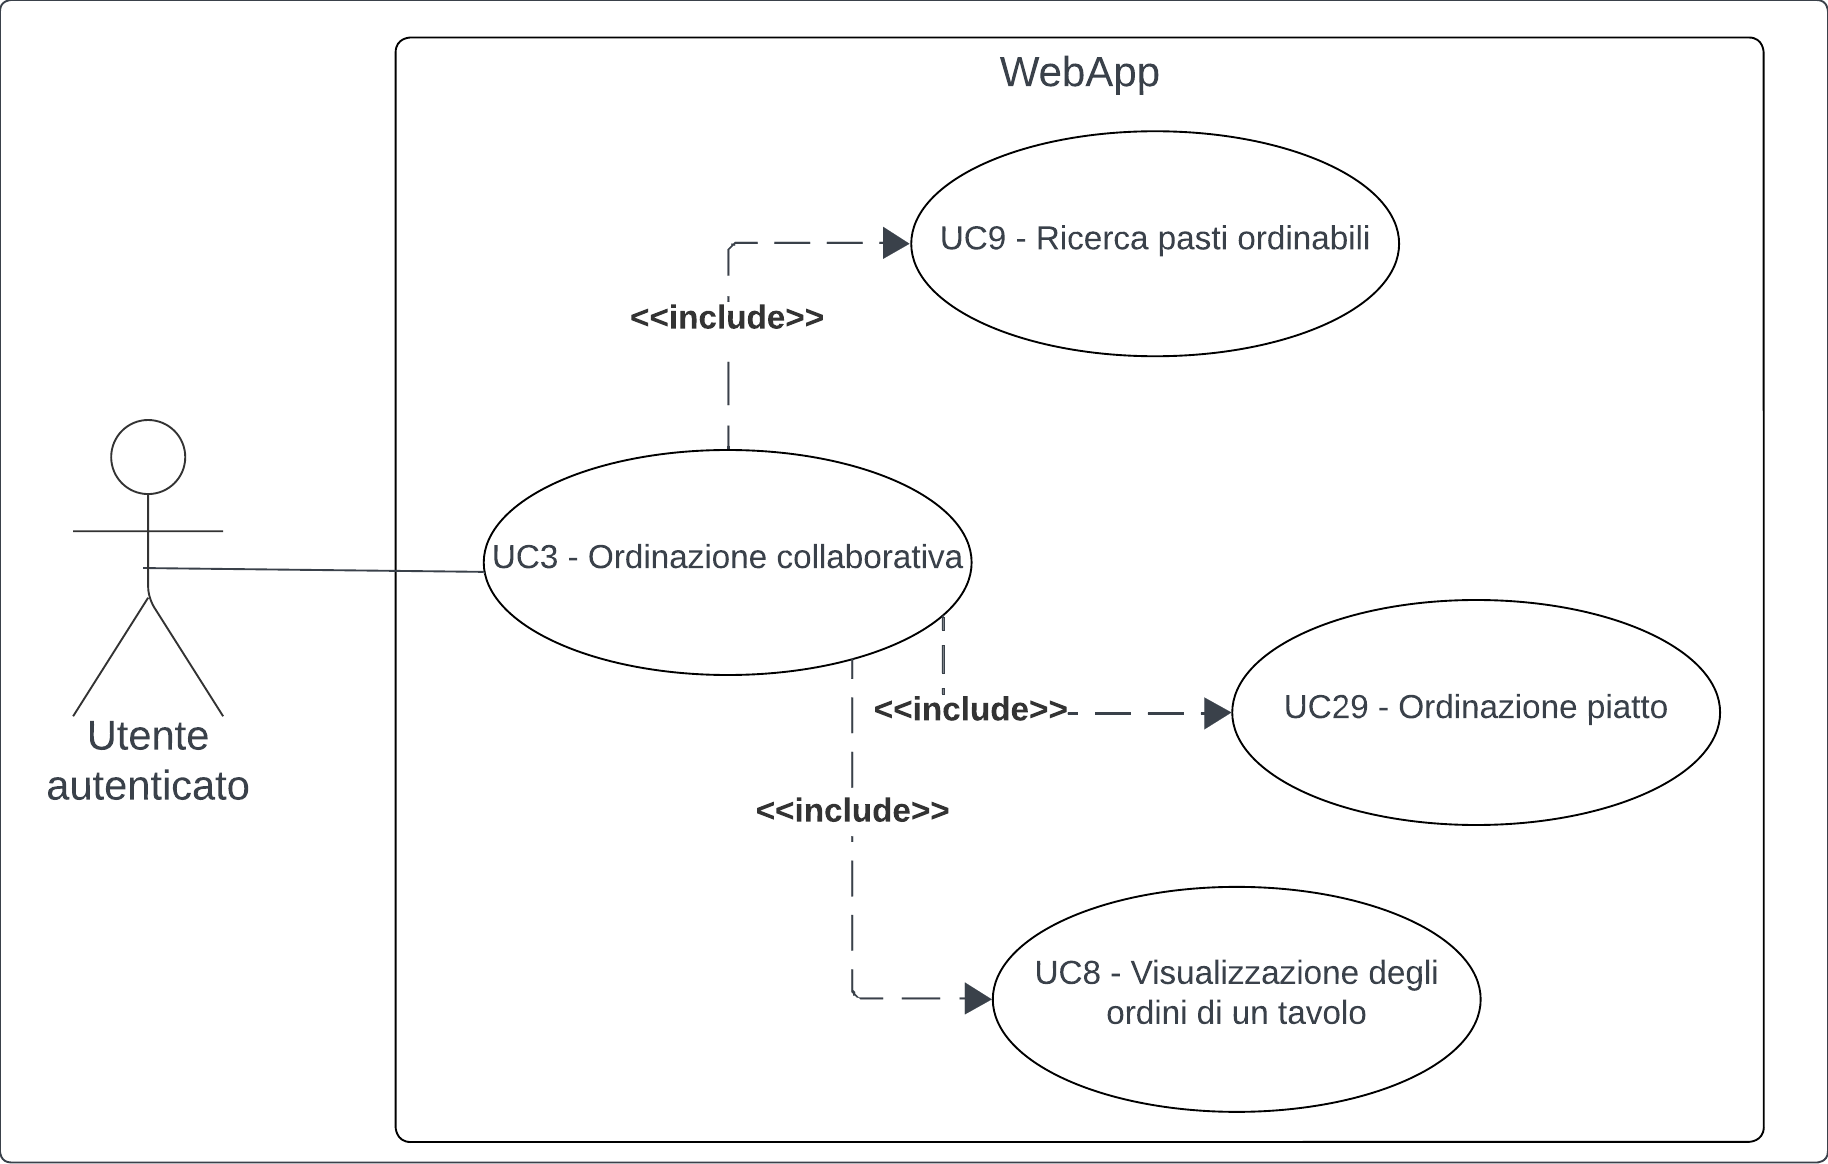
\includegraphics[width=0.9\linewidth]{ucd/UCD3.png}
\end{figure}

\textbf{Attori}:
\begin{itemize}
    \item Utente base autenticato
\end{itemize}
\textbf{Precondizioni}:
\begin{itemize}
    \item L'utente è autenticato dal $\textit{sistema}_G$ 
    \item L'utente ha prenotato un tavolo (\nameref{usecase:23})
    \item La $\textit{prenotazione}_G$ associata all'$\textit{ordinazione}_G$ è stata accettata dall'utente amministratore del ristorante (\nameref{usecase:19})
    \item Il tempo per l'$\textit{ordinazione}_G$ non è scaduto
\end{itemize}
\textbf{Postcondizioni}:
\begin{itemize}
    \item L'utente ha confermato l'$\textit{ordinazione}_G$ delle pietanze associata ad una $\textit{prenotazione}_G$.
\end{itemize}
\textbf{Scenario principale}:
\begin{enumerate}
    \item L'utente ricerca i pasti ordinabili (\nameref{usecase:9})
    \item L'utente sceglie il pasto da ordinare (\nameref{usecase:29}); nel caso in cui la pietanza ordinata contenga allergeni segnalati dall'utente in fase di registrazione, deve essere notificato prima di  aggiungere la pietanza all'ordine.
    \item L'utente può scegliere di: modificare la quantità degli ingredienti; rimuoverne alcuni ingredienti; aggiungere degli ingredienti (\nameref{usecase:29}).
    \item L'utente visualizza il riepilogo del suo ordine e quelli degli altri utenti con cui ha prenotato il tavolo (\nameref{usecase:8}).
    \item L'utente conferma l'$\textit{ordinazione}_G$.
    \item Il $\textit{sistema}_G$ notifica il ristorante mediante \textit{push-notification}.
\end{enumerate}
\newpage
\end{comment}